%% Copyright (C) 2009 EPITA Research and Development Laboratory (LRDE)
%%
%% This file is part of Olena.
%%
%% Olena is free software: you can redistribute it and/or modify it under
%% the terms of the GNU General Public License as published by the Free
%% Software Foundation, version 2 of the License.
%%
%% Olena is distributed in the hope that it will be useful,
%% but WITHOUT ANY WARRANTY; without even the implied warranty of
%% MERCHANTABILITY or FITNESS FOR A PARTICULAR PURPOSE.  See the GNU
%% General Public License for more details.
%%
%% You should have received a copy of the GNU General Public License
%% along with Olena.  If not, see <http://www.gnu.org/licenses/>.

\documentclass{article}

%\usepackage{hevea}

\usepackage{html}
\usepackage{hyperref}
\usepackage{graphicx}
\usepackage{makeidx}
\usepackage{xcolor}
\usepackage{color}

\title{Milena\\
  \large{Generic image processing library} }
\author{LRDE}
\date{}
\makeindex


\begin{document}

\maketitle

%#################################################################
\section{Introduction}
Milena is a programming framework for discrete mathematical morphology written
in C++. It is part of the Olena project which aims at building a scientific
computation platform oriented towards image processing, image recognition and
artificial vision.

Milena is designed with two major goals in mind:
\begin{itemize}
  \item Be as simple as calling C routines for end users.
  \item Be modular enough to be extended with respect to algorithms and data
	structures.
\end{itemize}


%#################################################################
\section{Targeted audience}
This library targets several audiences:
\begin{itemize}

  \item \textit{End users} of morphological tools who want to apply and assemble
  algorithms to solve image processing, pattern recognition or computer vision
  problems.
  \item \textit{Designers} of morphological operators who build new algorithms
  by using constructs from their software framework (language, livraries,
      toolboxes, programs, etc.).
  \item \textit{Providers} of data structures who are interested in extending
  their framework with new data types (images, values, structuring elements,
      etc.).

\end{itemize}

%#################################################################
\section{Key features}
Olena is:
\begin{itemize}
  \item \textbf{Generic}. If a morphological operator admis a general
	definition whatever the context (topology of the image, structuring
	element, etc.), then this algorithm should have a corresponding single
	implementation.

  \item \textbf{Close to theory}. Reading (and writing) algorithms should
	eventually become natural to scientists used to mathematical morphology
	notations.

  \item \textbf{Efficient} (with respect to run time speed and memory
	usage), when it is possible. Dedicated and efficient implementations of
	morphological algorithms for certain cases are known and should be
	selected whenever possible.

  \item \textbf{User-friendly}. Users should not have to address
	memory-related issues or deal with a program silently failing because of
	an arithmetic overflow. The tool should handle these situations, and
	help the user diagnose any problem.

  \item \textbf{Reliable}. Programming by contract helps debbuging user's
        programs. By default, a debug mode is enabled and check the data and
	access validity at runtime. Since Olena tends to be as static as
	possible, many static checks are also done at compile time.

  \item \textbf{Free}. Milena is \textit{free} and \textit{open-source}. It is
	released under GNU GPL V2.
\end{itemize}


%#################################################################
\section{Library content}

%=================================================================
\subsection{Generic basic image types}

Common basic image types are provided: 1-D, 2-D, 3-D images.
A $N$-D image class is also available.
These class are provided with a border in order to make them fast in algorithms
using structural elements.

%=================================================================
\subsection{Morphers}

Morphers are generic, composable and lightweight objects built on one or several
images, that can be used as
\begin{itemize}
  \item \textbf{mixins}: a morpher can add extra data (e.g. a neighborhood) or
	operations (e.g., an ordering on the values) to an image;
  \item \textbf{adapters}: e.g., a slice morpher can be used to view a slice of
	a 3-D image (spacemap) as a 2-D image (bitmap);
  \item \textbf{modifiers}: a morpher can add a mask to an image, to restrict its
	(iterable) domain;
  \item \textbf{lazy function applications}: a morpher can present an image seen
        through a function, either bijective or not;
  \item etc.
\end{itemize}

\begin{center}
  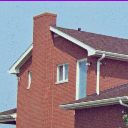
\includegraphics[width=2.5cm]{figures/house}%
  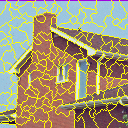
\includegraphics[width=2.5cm]{figures/house_wshed}%
  
\includegraphics[width=2.5cm]{figures/house_wshed_mean_colors}%
  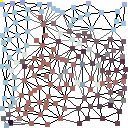
\includegraphics[width=2.5cm]{figures/house_rag}%
\end{center}

%=================================================================
\subsection{Generic image processing algorithms}

\begin{itemize}
  \item Morphological algorithms: dilation, erosion, watershed, leveling, etc;
  \item Influence zone;
  \item Labeling;
  \item etc.
\end{itemize}

%=================================================================
\subsection{Auxiliary tools}

Since Olena is intended to \textit{designer} of algorithms and \textit{provider}
of new data structures, various generic auxiliary tools are available in the
library.

\begin{itemize}
  \item Topologies (grid, graph, etc.);
  \item Points and delta-points;
  \item neighborhoods and windows;
  \item accumulators;
  \item etc.
\end{itemize}



%#################################################################
\section{Learn more}

Olena's \textbf{official website}: \url{http://olena.lrde.epita.fr}

Olena's \textbf{Trac}: \url{http://trac.lrde.org/olena}

Milena's \textbf{documentation}:
\url{http://www.lrde.epita.fr/dload/doc/milena/user-refman-html}

%
\medskip
%

\textbf{Mailing lists}:
\begin{itemize}
  \item olena@lrde.epita.fr - Question and comments;
  \item olena-bug@lrde.epita.fr - Bug reports;
  \item olena-patches@lrde.epita.fr - Patches.
\end {itemize}

%
\bigskip
%

\textbf{Contacts}:
\begin{itemize}
  \item Thierry Geraud - thierry.geraud@lrde.epita.fr
  \item Roland Levillain - roland.levillain@lrde.epita.fr
\end{itemize}

%Demo + tuto + doc


\section*{Copyright}
Copyright (C) 2009 EPITA Research and Development Laboratory (LRDE)

This document is part of Olena.

Olena is free software: you can redistribute it and/or modify it under
the terms of the GNU General Public License as published by the Free
Software Foundation, version 2 of the License.

Olena is distributed in the hope that it will be useful,
but WITHOUT ANY WARRANTY; without even the implied warranty of
MERCHANTABILITY or FITNESS FOR A PARTICULAR PURPOSE.  See the GNU
General Public License for more details.

You should have received a copy of the GNU General Public License
along with Olena.  If not, see $<$http://www.gnu.org/licenses/$>$.

\end{document}
